\documentclass[a4paper,10pt]{article}
\usepackage[utf8]{inputenc}

\usepackage{graphicx} % insert images
\usepackage{algorithm}
\usepackage{listings}
\usepackage{rotating}
\usepackage{epstopdf}
\graphicspath{{./figures/}}

%opening
\title{Guided Example using Mahout}
\author{Daniel Rodriguez\\\texttt{daniel.rodriguezg@uah.es}\\University of Alcala}

\date{}

\begin{document}

\maketitle

\section{Recommender System Example using Apache Mahout}


The implementation of the recommendation application of this project
required the following software.
\begin{itemize}
\item Maven (also using Eclipse, Netbeans, etc.)
\item A SQL Database (PostgreSQL, MySQL, etc.)
\item Apache Mahout libraries
\begin{itemize}
\item Apache Mahout Core
\item Apache Mahout Utils
\item Apache Mahout Math
\item Apache Mahout Collections
\end{itemize}
\end{itemize}


%\begin{center}
%\begin{figure}
%\begin{centering}
%\includegraphics[scale=0.5]{dependencyGraph.png}
%\par\end{centering}
%\caption{Dependency graph}
%\end{figure}
%\par\end{center}


%%%%%%%%%%%%%%%%%%%%%%%%%%%%%%%%%%%%%%%%%%%%%%%%%%%%%%%%%%%%%%%%%%%%%%
%%%%%%%%%%%%%%%%%%%%%%%%%%%%%%%%%%%%%%%%%%%%%%%%%%%%%%%%%% Intro

\section{Introducction}

\paragraph{}
This application example has been developed as a desktop Java application but it can be integrated (as a typical scenario) with Web server (e.g., Apache HTTP) or Web application servers
(Tomcat, Glassfish, etc.).

In this example datasets are stored in a SQL database (e.g. MySQL or PostgreSQL) and will be reached to
generate the model but also the library can access to a CSV file, etc. In fact in this example two flat files are generated from the database to be used by the recommender system algorithms (these file could be generated once a day or every few hours improve the performance). Also, depending on the architecture of the system, the performance results can change, for example, if the database is not located in the same computer as the application.

In order to install the libraries needed in the process, a library
manager is used to download it automatically (Maven). This tool also allows
us to export the application to other system easily.


\subsection{Architecture}

This example project is composed of for core files:

\begin{itemize}
    \item \texttt{App.java}: This is the main class. This class just creates an instance
    of the ``recommend'' class to print the results.
    \item \texttt{DBManager.java}: This class creates the connection to the database. It also contains some methods to retrieve the data and create a CSV file with the result set.
    \item \texttt{RecommenderSamples.java}: It contains the algorithms to get the recommendations
    (all 4 of the algorithms included in the library).
    \item \texttt{jdbc.properties}: To set the details of the database connection.
\end{itemize}

These classes need other libraries to work, manage the database or create the recommendations. However, they are managed with ``Apache Maven'' which facilitates their installation process and is generally integrated in IDEs. We just needed to create a dependency file to attach our libraries to the project. This file is an XML (POM\footnote{\texttt{http://maven.apache.org/pom.html}}) file which looks for the libraries used in a central server to download

\begin{lstlisting}[basicstyle={\scriptsize},breaklines=true,language=XML,
numbers=left,numberstyle={\scriptsize},tabsize=4]
  <dependencies>
        <dependency>
			<groupId>postgresql</groupId>
			<artifactId>postgresql</artifactId>
			<version>9.1-901.jdbc4</version>
		</dependency>
        <dependency>
            <groupId>mysql</groupId>
            <artifactId>mysql-connector-java</artifactId>
            <version>5.1.25</version>
        </dependency>
        <dependency>
            <groupId>org.apache.mahout</groupId>
            <artifactId>mahout-math</artifactId>
            <version>0.7</version>
        </dependency>
        <dependency>
            <groupId>org.apache.mahout</groupId>
            <artifactId>mahout-collections</artifactId>
            <version>1.0</version>
        </dependency>
        <dependency>
            <groupId>org.apache.mahout</groupId>
            <artifactId>mahout-core</artifactId>
            <version>0.7</version>
        </dependency>
        <dependency>
            <groupId>org.apache.mahout</groupId>
            <artifactId>mahout-utils</artifactId>
            <version>0.5</version>
        </dependency>
        <dependency>
            <groupId>org.apache.mahout</groupId>
            <artifactId>mahout-buildtools</artifactId>
            <version>0.7</version>
        </dependency>
    </dependencies>
\end{lstlisting}

%%%%%%%%%%%%%%%%%%%%%%%%%%%%%%%%%%%%%%%%%%%%%%%%%%%%%%%%%%%%%%%%%%%%%%

\subsection{Datasets}

One of the important issue before generating recommendations is
the dataset. Our dataset is stored in a relational database in 2 different
tables:

\begin{itemize}
\item ContentRatings: This table contains the ratings given by the users
to a determined content. This table stores the following fields (figure
\ref{fig:Content-table}):

\begin{itemize}
\item idcontent: The identifier of the content rated
\item Rating: Value from 1 to 5 given by the user to measure the content
\item Date: Unix time when the rating was made.
\item fromUser: Identifier of the user who made the rating.
\item hashedId: The identifier of the content encoded with MD5 algorithm.
This identifier is encoded because Mahout works easier with numeric
id's.
\end{itemize}
\end{itemize}


\begin{center}
\begin{figure}
\begin{centering}
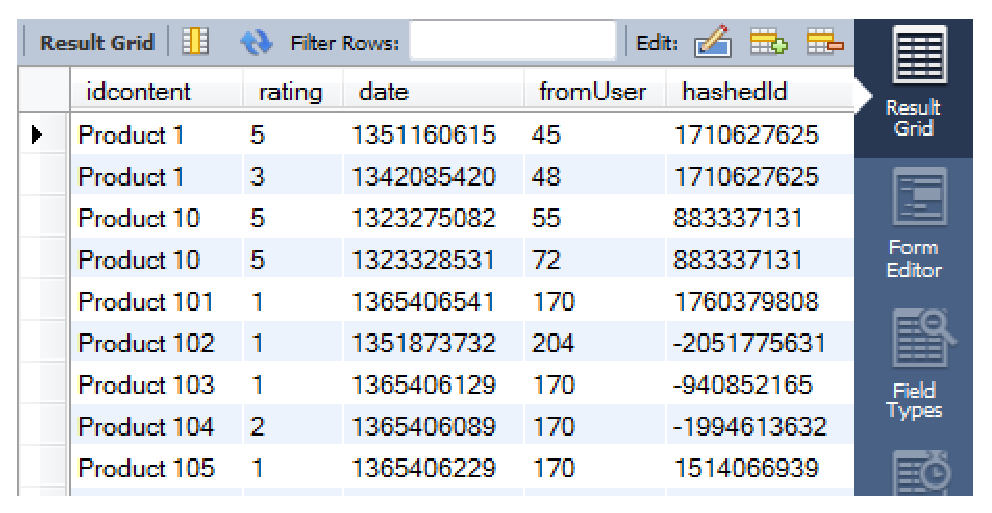
\includegraphics[scale=0.6]{content.eps}
\par\end{centering}
\caption{Content table\label{fig:Content-table}}
\end{figure}

\par\end{center}
\begin{itemize}


\item UserRatings: Contains the ratings given by the users to other users
(figure \ref{fig:Users-table}):

\begin{itemize}
\item iduser: Identifier of the user rated.
\item rating: Value from 1 to 5 to measure the user.
\item date: Unix time when the rating was made.
\item fromUser: Identifier of the user who made the rating.
\end{itemize}
\end{itemize}


\begin{center}
\begin{figure}%
\begin{centering}
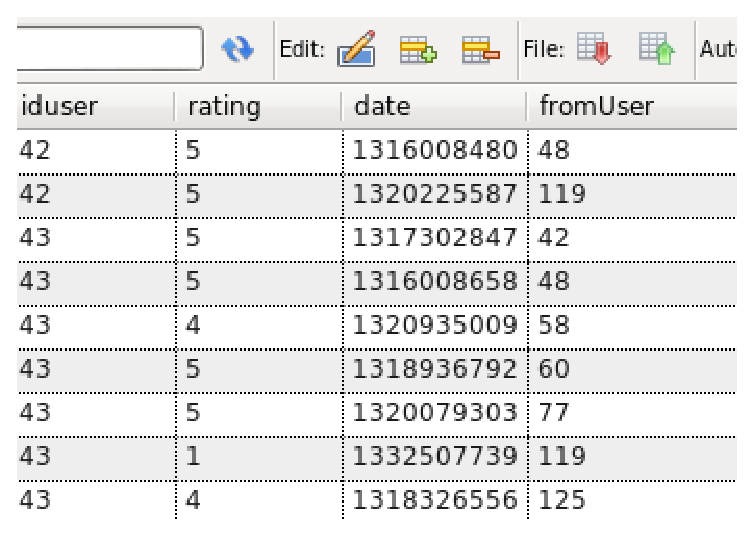
\includegraphics[scale=0.6]{users}
\par\end{centering}
\caption{Users table\label{fig:Users-table}}
\end{figure}
\par\end{center}


%%%%%%%%%%%%%%%%%%%%%%%%%%%%%%%%%%%%%%%%%%%%%%%%%%%%%%%%%%%%%%%%%%%%%%%%%%%%%%%
\subsection{Example}

The example application shows four different recommendation algorithms:

\begin{enumerate}
    \item Slope One for users
    \item Nearest neighbourhood for users
    \item Slope One for items
    \item Nearest neighbourhood for items
\end{enumerate}

The application runs all four algorithms to get the recommendations and to compare them (in practice only there is no need to run multiple algorithms). The application can be easily configured by a configuration file that contains the information to access to the database, etc.


\begin{lstlisting}[basicstyle={\small},breaklines=true,language=XML,numbers=left
,numberstyle={\footnotesize}]
jdbc.driverClassName = com.mysql.jdbc.Driver
jdbc.databaseUrl = jdbc:mysql://localhost/ratings
jdbc.username = root
jdbc.password = password
\end{lstlisting}



When the application is executed, takes the data from the database
and the method ``createDbFile'' of the class ``dataBaseHandler''
stores it in a temporal file. This file is created to avoid performance
problems when the dataset is too large.

In order to control whether
the ratings file is updated, the date (in UNIX time format%
\footnote{http://en.wikipedia.org/wiki/Unix\_time%
}) of last check is stored in the fields: \texttt{suggestUsers.dat} and
\texttt{suggestContent.dat}.
In practice the application should be extended with code to control the interval of the file can be easily managed in the application changing one parameter.

%%%%%%%%%%%%%%%%%%%%%%%%%%%%%%%%%%%%%%%%%%%%%%%%%%%%%%%%%%%%%%%%%%%%%%%%%%%%%%%
%

\section{Results: Recommend users algorithms}

These algorithms will recommend users or friends to a given user.
In this case we have executed the application with 2 different algorithms
to check the differences between them:

\begin{enumerate}
\item Slope One for users.
\item Nearest neighbourhood for users.
\end{enumerate}

The initial conditions for the test are:
\begin{itemize}
\item Identifier of the user to recommend friends: 45.
\item Number of requested users: 8.
\item Neighbourhood: 10.
\end{itemize}


The results of the execution are:

\begin{center}
\begin{figure}[H]
\begin{centering}
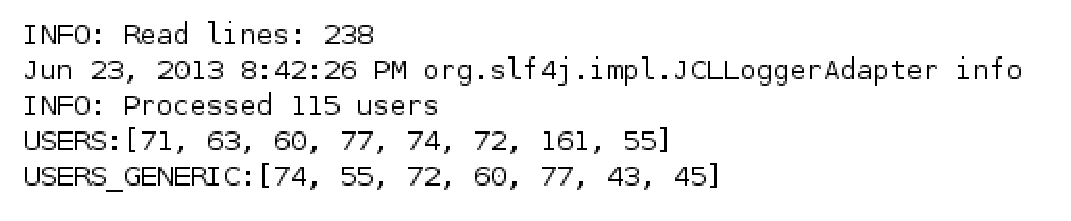
\includegraphics[scale=0.55]{userRecommendation.eps}
\par\end{centering}

\caption{Users recommendation result $K$=10}
\end{figure}

\par\end{center}

The dataset used is composed of 238 rating of users and 115 different users.

The Slope One algorithm returned the users: 71, 63, 60, 77,
74, 72, 161 and 55.

The $kNN$ algorithm returned users: 74, 55, 72, 60, 77, 43 and 45.

%This algorithm returned only 7 users and one of them is the user 45, probably due to a short dataset or a non adequate number of neighborhoods.

%%%%%%%%%%%%%%%%%%%%%%%%%%%%%%%%%%%%%%%%%%%%%%%%%%%%%%%%%%%%%%%%%%
\section{Exercises}

\begin{itemize}
  \item Try with different number of neighbours.
  \item Compare the results of the item-based and user-based algorithms.
\end{itemize}


\end{document}
